%\vspace{-5pt}
\section{Study}
\label{sec:study}

To understand how programmers use regular expressions in Python projects, we scraped \DTLfetch{data}{key}{nProjScanned}{value} Python projects from GitHub, and recorded regex usages for analysis. Throughout the rest of this paper, we  employ the following terminology:\\

\noindent \textbf{Utilization}: A \emph{utilization} occurs whenever a regex appears in source code.  We detect utilizations by statically analyzing the code and recording calls to the {\tt re} module in Python.
Within a particular file in a project, a {utilization} is composed of a function, a pattern, and 0 or more flags.  Figure~\ref{fig:exampleUsage} presents an example of one regex {utilization}, with key components labeled. The function call is {\tt re.compile}, \verb!(0|-?[1-9][0-9]*)$! is the regex string, or pattern, and {\tt re.MULTILINE} is an (optional) flag. This {utilization}  will compile a regex object in the variable {\tt r1} from the pattern \verb!(0|-?[1-9][0-9]*)$!, with the \verb!$! token matching at the end of each line because of the {\tt re.MULTILINE} flag. Thought of another way, a regular expression  utilization is one single invocation of the {\tt re} library.\\

\begin{figure}[tb]
\centering
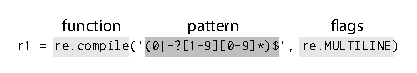
\includegraphics[width=\columnwidth]{../illustrations/exampleUsage.eps}
\vspace{-6pt}
\caption{Example of one regex utilization}
\vspace{-6pt}
\label{fig:exampleUsage}
\end{figure}

\noindent \textbf{Pattern}: A \emph{pattern} is extracted from a utilization, as shown in Figure~\ref{fig:exampleUsage}. In essence, it is a string, but more formally it is an ordered series of regular expression language feature tokens.  The pattern in Figure~\ref{fig:exampleUsage}  will match if it finds a zero at the end of a line, or a (possibly negative) integer at the end of a line (i.e., due to the {\tt -?} sequence denoting zero or one instance of the {\tt -}).

Note that because the vast majority of regex features are shared across most general programming languages (e.g., Java, C, C\#, or Ruby), a Python {pattern} will (almost always) behave the same when used in other languages, whereas a utilization is not universal in the same way (i.e., it may not compile in other languages, even with small modifications to function and flag names).
As an example, the {\tt re.MULTILINE} flag, or similar, is present in Python, Java, and C\#, but  the Python {\tt re.DOTALL} flag is not present in C\# though it has an equivalent flag in Java.

In this work, we primarily focus on patterns since they are cross-cutting across languages and are the primary way of specifying the matching behavior. Next, we describe the research questions, data set collection and analysis. 

\subsection{Research Questions}
\label{sec:rqs}
To understand the contexts in which regular expressions are used  and feature usage, we perform a survey of developers and explore regular expressions found in Python projects on GitHub. We aim to answer the following research questions:\\

\noindent \textbf{RQ1:} In what contexts do professional developers use regular expressions?

We designed and deployed a survey about when, why, and how often they use regular expressions. This was completed by 18 professional developers at a small software company.\\

\noindent \textbf{RQ2:} How  is the {\tt re} module used in Python projects?

We explore invocations of  the {\tt re} module in \DTLfetch{data}{key}{nProjScanned}{value} Python projects scraped from GitHub.\\


\noindent \textbf{RQ3:} Which regular expression language features are most commonly used in Python?

We consider regex language features to be tokens that specify the matching behavior of a regex pattern, for example,  the {\tt +} in {\tt ab+}.  All studied features are listed and described in Section~\ref{study:corpus} with examples. We then map the feature coverage for four common regex support tools, brics, hampi, RE2 and Rex, and explore survey responses regarding feature usage for some of the less supported features.\\

\noindent \textbf{RQ4:} How behaviorally similar are regexes across projects?

As this is a first step in understanding behavioral overlap in
regexes, we measure similarity between pairs of regexes by overlap in matching strings. For each regex, matching strings are generated and then  evaluated against each other regex to compute pairwise similarity. Then we use clustering to form behaviorally similar groupings. 


%\noindent \textbf{RQ5:} What is the impact of \emph{not} supporting various regular expression features on tool users and designers?
%
%We use semantic analysis to illustrate the impact of missing features on a tool's applicability by identifying what each feature (or group of features) is commonly used for. \\

%Next, we describe our survey, how the corpus of regex patterns was built, how features were analyzed, and how the clustering was performed.

\subsection{Survey Design and Implementation}
\label{study:survey}
To understand the context of when and how programmers use regular expressions, 
we designed a survey, implemented using Google Forms, with 40 questions. The questions asked about regex usage frequency, languages, purposes, pain points, and the use of various language features.\footnote{\url{https://github.com/softwarekitty/tour_de_source/blob/master/regex_usage_in_practice_survey.pdf}}  Participation was voluntary and participants were entered in a lottery for a \$50 gift card. 

Our goal was to understand the practices of professional developers. Thus, we deployed the survey to 22 professional developers at Dwolla, a small software company that provides tools for online and mobile payment management. While this sample comes from a single company, we note anecdotally that Dwolla is a start-up and most of the developers worked previously for other software companies, and thus bring their past experiences with them. Surveyed developers have nine years of experience, on average, indicating the results may generalize beyond a single, small software company, but further study is needed. 


%The questions asked about regex usage frequency, languages, purposes, and the use of various language features, as explored in Section~\ref{rq1:survey} and Section~\ref{results:rq3}. 
%\todoMid{More details on survey design}


\subsection{Regex Corpus}
\label{study:corpus}
Our goal was to collect regexes from a variety of projects to represent the breadth of how developers use the language features. 
Using the GitHub API, we scraped \DTLfetch{data}{key}{nProjScanned}{value}  projects containing Python code.  
We did so  by dividing a range of about 8 million repo IDs for Python projects
into 32 sections of equal size and scanning from the beginning of those
segments until we ran out of memory. At that point, we felt we had enough data
to do an analysis without further perfecting our mining techniques. We built
the AST of each file in each project to find utilizations of the 're' module
functions. In most projects, almost all regex utilizations are present in the
most recent version of a project, but to be more thorough, we also scanned up
to 19 earlier versions. The number 20 was chosen to try and maximize returns on
computing resources invested after observing the scanning process in many hours
of trial scans.
% If the project had fewer than 20 commits, then all commits were scanned.  
% The most recent commit was always included, and the spacing between all other chosen commits was determined by dividing the remaining number of commits by 19 (rounding as needed).
All regex utilizations were obtained, sans duplicates. Within a project, a duplicate utilization was marked when two versions of the same file have the same function, pattern and flags.  In the end, we observed and recorded \DTLfetch{data}{key}{nUsages}{value} non-duplicate regex utilizations in \DTLfetch{data}{key}{nProjScanned}{value} projects.

In collecting the set of distinct patterns for analysis,  we ignore the \DTLfetch{data}{key}{percentBadFlags}{value}\%  of utilizations using flags, which can alter regex behavior.  An additional \DTLfetch{data}{key}{percentInvalidPattern}{value}\% of utilizations contained patterns that could not be compiled because the pattern was non-static (e.g., used some runtime variable).
The remaining \DTLfetch{data}{key}{percentCleanUsages}{value}\% (\DTLfetch{data}{key}{nCleanUsages}{value}) of the utilizations were collapsed into \DTLfetch{data}{key}{nDistinctPatterns}{value} distinct pattern strings.  Each of the pattern strings was pre-processed by removing Python quotes (\verb!`\\W!' becomes \verb!\\W!), unescaping escaped characters (\verb!\\W! becomes \verb!\W!) and parsing the resulting  string using an ANTLR-based, open source PCRE parser\footnote{\url{https://github.com/bkiers/pcre-parser}}.
This parser was unable to support \DTLfetch{data}{key}{percentUnicode}{value}\% (\DTLfetch{data}{key}{N_UNICODE}{value}) of the patterns due to unsupported unicode characters.  Another \DTLfetch{data}{key}{percentAlien}{value}\% (\DTLfetch{data}{key}{N_ALIEN}{value}) of the patterns used regex features that we  chose to exclude because appeared very rarely (e.g., reference conditions).

The \DTLfetch{data}{key}{nCorpus}{value} distinct pattern strings that remain were each assigned a weight value equal to the number of distinct projects the pattern appeared in.  We  refer to this set of weighted, distinct pattern strings as the \emph{corpus}.

\subsection{Analyzing Features}
\label{study:features}
For each escaped pattern, the PCRE-parser produces a tree of feature tokens, which is converted to a vector by counting the number of each token present in the tree.  For a simple example, consider the patterns in Figure~\ref{fig:featureParsing}.  The pattern \verb!`^m+(f(z)*)+'! contains four different types of tokens. It contains the kleene star (KLE), which is specified using the asterisk \verb!`*'! character, additional repetition (ADD), which is specified using the plus \verb!`+'! character, capture groups (CG), which are specified using pairs of parenthesis \verb!`(...)'! characters, and the start anchor (STR), which is specified using the caret \verb!`^'! character at the beginning of a pattern.

\begin{figure}[tb]
\centering
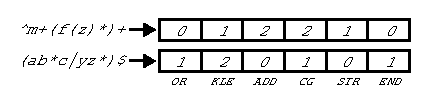
\includegraphics[height=0.6in]{../illustrations/featureParsing.eps}
\caption{Two patterns parsed into feature vectors}
\label{fig:featureParsing}
\vspace{-12pt}
\end{figure}

Once all patterns were transformed into vectors, we examined each feature independently for all patterns, tracking the number of patterns and  projects that the each feature appears in at least once.




\subsection{Clustering and Behavioral Similarity}
An ideal analysis of similarity for regexes would use subsumption or containment analysis. However, we struggled to find a tool that could facilitate such an analysis. Further, regular expressions in modern code libraries are not the same as regular languages in formal language theory. Some features of regular expression libraries, such as backreferences,  provide expressiveness beyond regular languages. This allows a regular expression pattern to match, for example, repeat words, such as ``cabcab", using the pattern {\tt (.+)\verb!\!1}. However, building an automaton to recognize such a pattern and to facilitate containment analysis, is infeasible. 
For these reasons, we developed a similarity analysis based on string matching. 


\begin{figure}[tb]
\centering
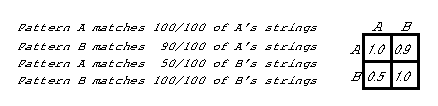
\includegraphics[height=0.6in]{../illustrations/minimalMatrix.eps}
\caption{A similarity matrix created by counting strings matched}
\label{fig:minimalMatrix}
\end{figure}


\begin{figure}[tb]
\centering
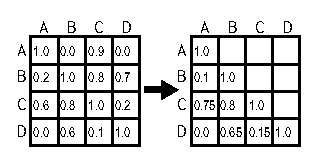
\includegraphics[width=0.7\columnwidth]{../illustrations/matrixToGraph.eps}
\vspace{-6pt}
\caption{Creating a similarity graph from a similarity matrix}
\vspace{-6pt}
\label{fig:matrixToGraph}
\end{figure}

Our similarity analysis clusters regular expressions by their behavioral similarity on matched strings.
Consider two unspecified patterns {\tt A} and {\tt B}, a set {\tt mA} of 100 strings that pattern {\tt A} matches, and a set {\tt mB} of 100 strings that pattern {\tt B} matches.
If pattern {\tt B} matches 90 of the 100 strings in the set {\tt mA}, then {\tt B} is 90\% similar to {\tt A}.
If pattern {\tt A} only matches 50 of the strings in {\tt mB}, then {\tt A} is 50\% similar to {\tt B}.
We use similarity scores to create a similarity matrix as shown in Figure~\ref{fig:minimalMatrix}.
In row {\tt A}, column {\tt B} we see that {\tt B} is 90\% similar to {\tt A}.
In row {\tt B}, column {\tt A}, we see that {\tt A} is 50\% similar to {\tt B}.  Each pattern is always 100\% similar to itself, by definition.

Once the similarity matrix is built, the values of cells reflected across the diagonal of the matrix are averaged to create a half-matrix of undirected similarity edges, as illustrated in Figure~\ref{fig:matrixToGraph}.
This facilitates clustering using the  Markov Clustering (MCL) algorithm\footnote{\url{http://micans.org/mcl/}}.
We chose MCL  because it offers a fast and tunable way to cluster items by similarity and it is particularly useful when the number of clusters is not known \emph{a priori}.


In the implementation, strings are generated for each pattern using Rex~\cite{rex}.  Rex generates matching strings by representing the regular expression as an automaton, and then passing that automation to a constraint solver that generates members for it\footnote{\url{http://research.microsoft.com/en-us/projects/rex/}}.  If the regex matches a finite set of strings smaller than 400, Rex will produce a list of all possible strings.
Our goal is to generate 400 strings for each pattern to balance the runtime of the similarity analysis with the precision of the similarity calculations.


For clustering, we prune the similarity matrix to retain all similarity values greater than or equal to 0.75, setting the rest to zero, and then using MCL.
This threshold was selected based on recommendations in the MCL manual. The impact of lowering the threshold would likely result  in either the same number of more diverse clusters, or a larger number of clusters, but is unlikely to markedly change the largest clusters or their summaries, which are the focus of our analysis for RQ4 (Section~\ref{rq4:results}), but further study is needed to substantiate this claim. 
We also note that MCL can be tuned using many parameters, including inflation and filtering out all but the top-k edges for each node.
After exploring the quality of the clusters using various tuning parameter combinations, the best clusters (by inspection) were found using an inflation value of 1.8 and k=83.   The top 100 clusters are categorized by inspection into six categories of behavior. % (see Section~\ref{rq4:results}).

The end result is clusters and categories of highly behaviorally similar regular expressions, though we note that this approach has a tendency to over-approximate the similarity of two regexes. We measure similarity based on a finite set of generated strings, but some regexes  match an infinite set (e.g., \verb!ab*c!), so measuring similarity based on the first 400 strings may lead to an artificially high similarity value. To mitigate this threat, we chose a large number of generated strings for each regex.


%\todoNow{fix this before the ICSE deadline - after putting several days into this, I have a partial fix but the fact is there was information loss when going between the java program and the cs program and back again.  So it remains to be seen if it will be feasible to do non-automatic repairs.}
%
%
%We note that there was an operational error in pulling patterns from our database prior to the similarity analysis and clustering, so that 224 patterns (2.3\%) of the 9,727 patterns were omitted. These were duplicate patterns that were quoted differently (for example \verb!`\W'! and \verb!"\W"!).  The result of this error is a slight underestimate in number of projects per pattern (and per cluster), and a slight over-estimate in the pattern, file and project statistics shown in Table~\ref{table:featureStats}.  We do not believe that this error affects our conclusions.

